\title{ALPSチュートリアル -- ALPSのインストール}

\begin{document}

\begin{frame}
  \titlepage
\end{frame}

\section*{Outline}
\begin{frame}
  \tableofcontents
\end{frame}

\section{ALPSがインストールされているシステム}
\begin{frame}[fragile]
  \frametitle{ALPSがインストールされているシステム}
  \begin{itemize}
  \item 物性研システムB (kashiwa), システムC (maki)
  \item 京 (k)
  \item 東大FX10 (oakleaf-fx)
  \item 京大Cray XE6 (camphor)
  \item 九大X86クラスタ (tatara)
  \item ...
  \item 他にも順次インストール中 (アカウントをいただければ出張インストールします)
  \end{itemize}
\begin{semiverbatim}
参考: {\footnotesize \url{https://github.com/wistaria/installer/wiki}}
\end{semiverbatim}
\end{frame}

\section{ALPSのインストール}
\begin{frame}
  \frametitle{ALPSの依存関係}
  \begin{itemize}
  \item<1-> 必須のもの\\
    \begin{tabular}{ll}
      CMake & \url{http://www.cmake.org/} \\
      Boost & \url{http://www.boost.org/} \\
      HDF5  & \url{http://www.hdfgroup.org/HDF5/} \\
      BLAS/LAPACK & \url{http://www.netlib.org/} \\
    \end{tabular}
  \item<2-> 結果の解析に必要なもの \\
    \begin{tabular}{ll}
      Python & \url{http://www.python.org/} \\
      Numpy & \url{http://www.numpy.org} \\
      Scipy & \url{http://www.scipy.org} \\
      Matplotlib & \url{http://matplotlib.org/}
    \end{tabular}
  \item<3-> あるとよいもの \\
    \begin{tabular}{ll}
      MPI & \url{http://www.mpi-forum.org/} \\
    \end{tabular}
  \end{itemize}
\end{frame}

\begin{frame}[fragile,shrink=10]
  \frametitle{Debian系Linuxでのインストール}
  \begin{enumerate}
  \item 必要なライブラリをapt-getする
\begin{semiverbatim}
# apt-get install cmake-curses-gui libhdf5-dev liblapack-dev mpi-default-dev
# apt-get install python-matplotlib python-scipy
\end{semiverbatim}
  \item ALPSのビルドとインストール
\begin{semiverbatim}
\$ wget http://exa.phys.s.u-tokyo.ac.jp/archive/source/\\
  alps-20140524-r7462.tar.gz
\$ wget http://sourceforge.net/projects/boost/files/\\
  boost/1.54.0/boost_1_54_0.tar.bz2
\$ tar zxf alps-20140524-r7462.tar.gz
\$ tar jxf boost_1_54_0.tar.bz2
\$ mkdir build && cd build
\$ cmake -DBoost_ROOT_DIR=$HOME/boost_1_54_0 \\
  $HOME/alps-20140524-r7462
\$ make && ctest && make install
\end{semiverbatim}
  \end{enumerate}
\end{frame}

\begin{frame}[fragile,shrink=10]
  \frametitle{Mac OS X (Marvericks)でのインストール}
  \begin{enumerate}
  \item 必要なライブラリを\href{http://www.macports.org/}{MacPorts}からインストール
\begin{semiverbatim}
\$ sudo port install gcc48
\$ sudo port select --set gcc mp-gcc48
\$ sudo port install openmpi-gcc48
\$ sudo port select --set mpi openmpi-gcc48-fortran
\$ sudo port install python27 py27-ipython py27-scipy py27-matplotlib
\$ sudo port install cmake hdf5-18 +threadsafe wget
\end{semiverbatim}
  \item ALPSのビルドとインストール
\begin{semiverbatim}
\$ wget http://exa.phys.s.u-tokyo.ac.jp/archive/source/\\
  alps-20140524-r7462.tar.gz
\$ wget http://sourceforge.net/projects/boost/files/\\
  boost/1.54.0/boost_1_54_0.tar.bz2
\$ tar zxf alps-20140524-r7462.tar.gz
\$ tar jxf boost_1_54_0.tar.bz2
\$ mkdir build && cd build
\$ vi alps-cmake.sh (see next page)
\$ sh alps-cmake.sh
\$ make && ctest && make install
\end{semiverbatim}
  \end{enumerate}
\end{frame}

\begin{frame}[fragile,shrink=10]
 \frametitle{Mac OS X用のCMakeの設定例 (alps-cmake.sh)}
 \begin{semiverbatim}
#!/bin/bash
PREFIX=${HOME}/opt/alps
ALPS_SRC=${HOME}/sources/archive/alps-20140524-r7462
BOOST_SRC=${HOME}/sources/archive/boost_1_54_0

cmake -DCMAKE_INSTALL_PREFIX=${PREFIX} \\
  -DCMAKE_BUILD_TYPE=Release \\
  -DCMAKE_CXX_COMPILER=g++ -DCMAKE_C_COMPILER=gcc \\
  -DCMAKE_Fortran_COMPILER=gfortran -DALPS_BUILD_FORTRAN=ON \\
  -DBoost_ROOT_DIR=${BOOST_SRC} \\
  -DALPS_ENABLE_OPENMP=ON -DALPS_ENABLE_OPENMP_WORKER=ON \\
  -DPYTHON_INTERPRETER=python2.7 \\
  ${ALPS_SRC}
 \end{semiverbatim}
\end{frame}

\section{MateriApps}

\begin{frame}
 \frametitle{MateriApps}
 \begin{itemize}
   \item USBメモリから直接ブートできる Linux システム (Debian Live)
   \item 代表的な物質科学公開ソフト・ツールがあらかじめインストールされている
   \item 2014年3月現在:ABINIT, ALPS, CP2K, Feram ,ERmod, GAMESS, Gromacs, AkaiKKR, OpenMX, Quantum Espresso, xTAPP (順次追加予定)
     \hspace*{7cm}
     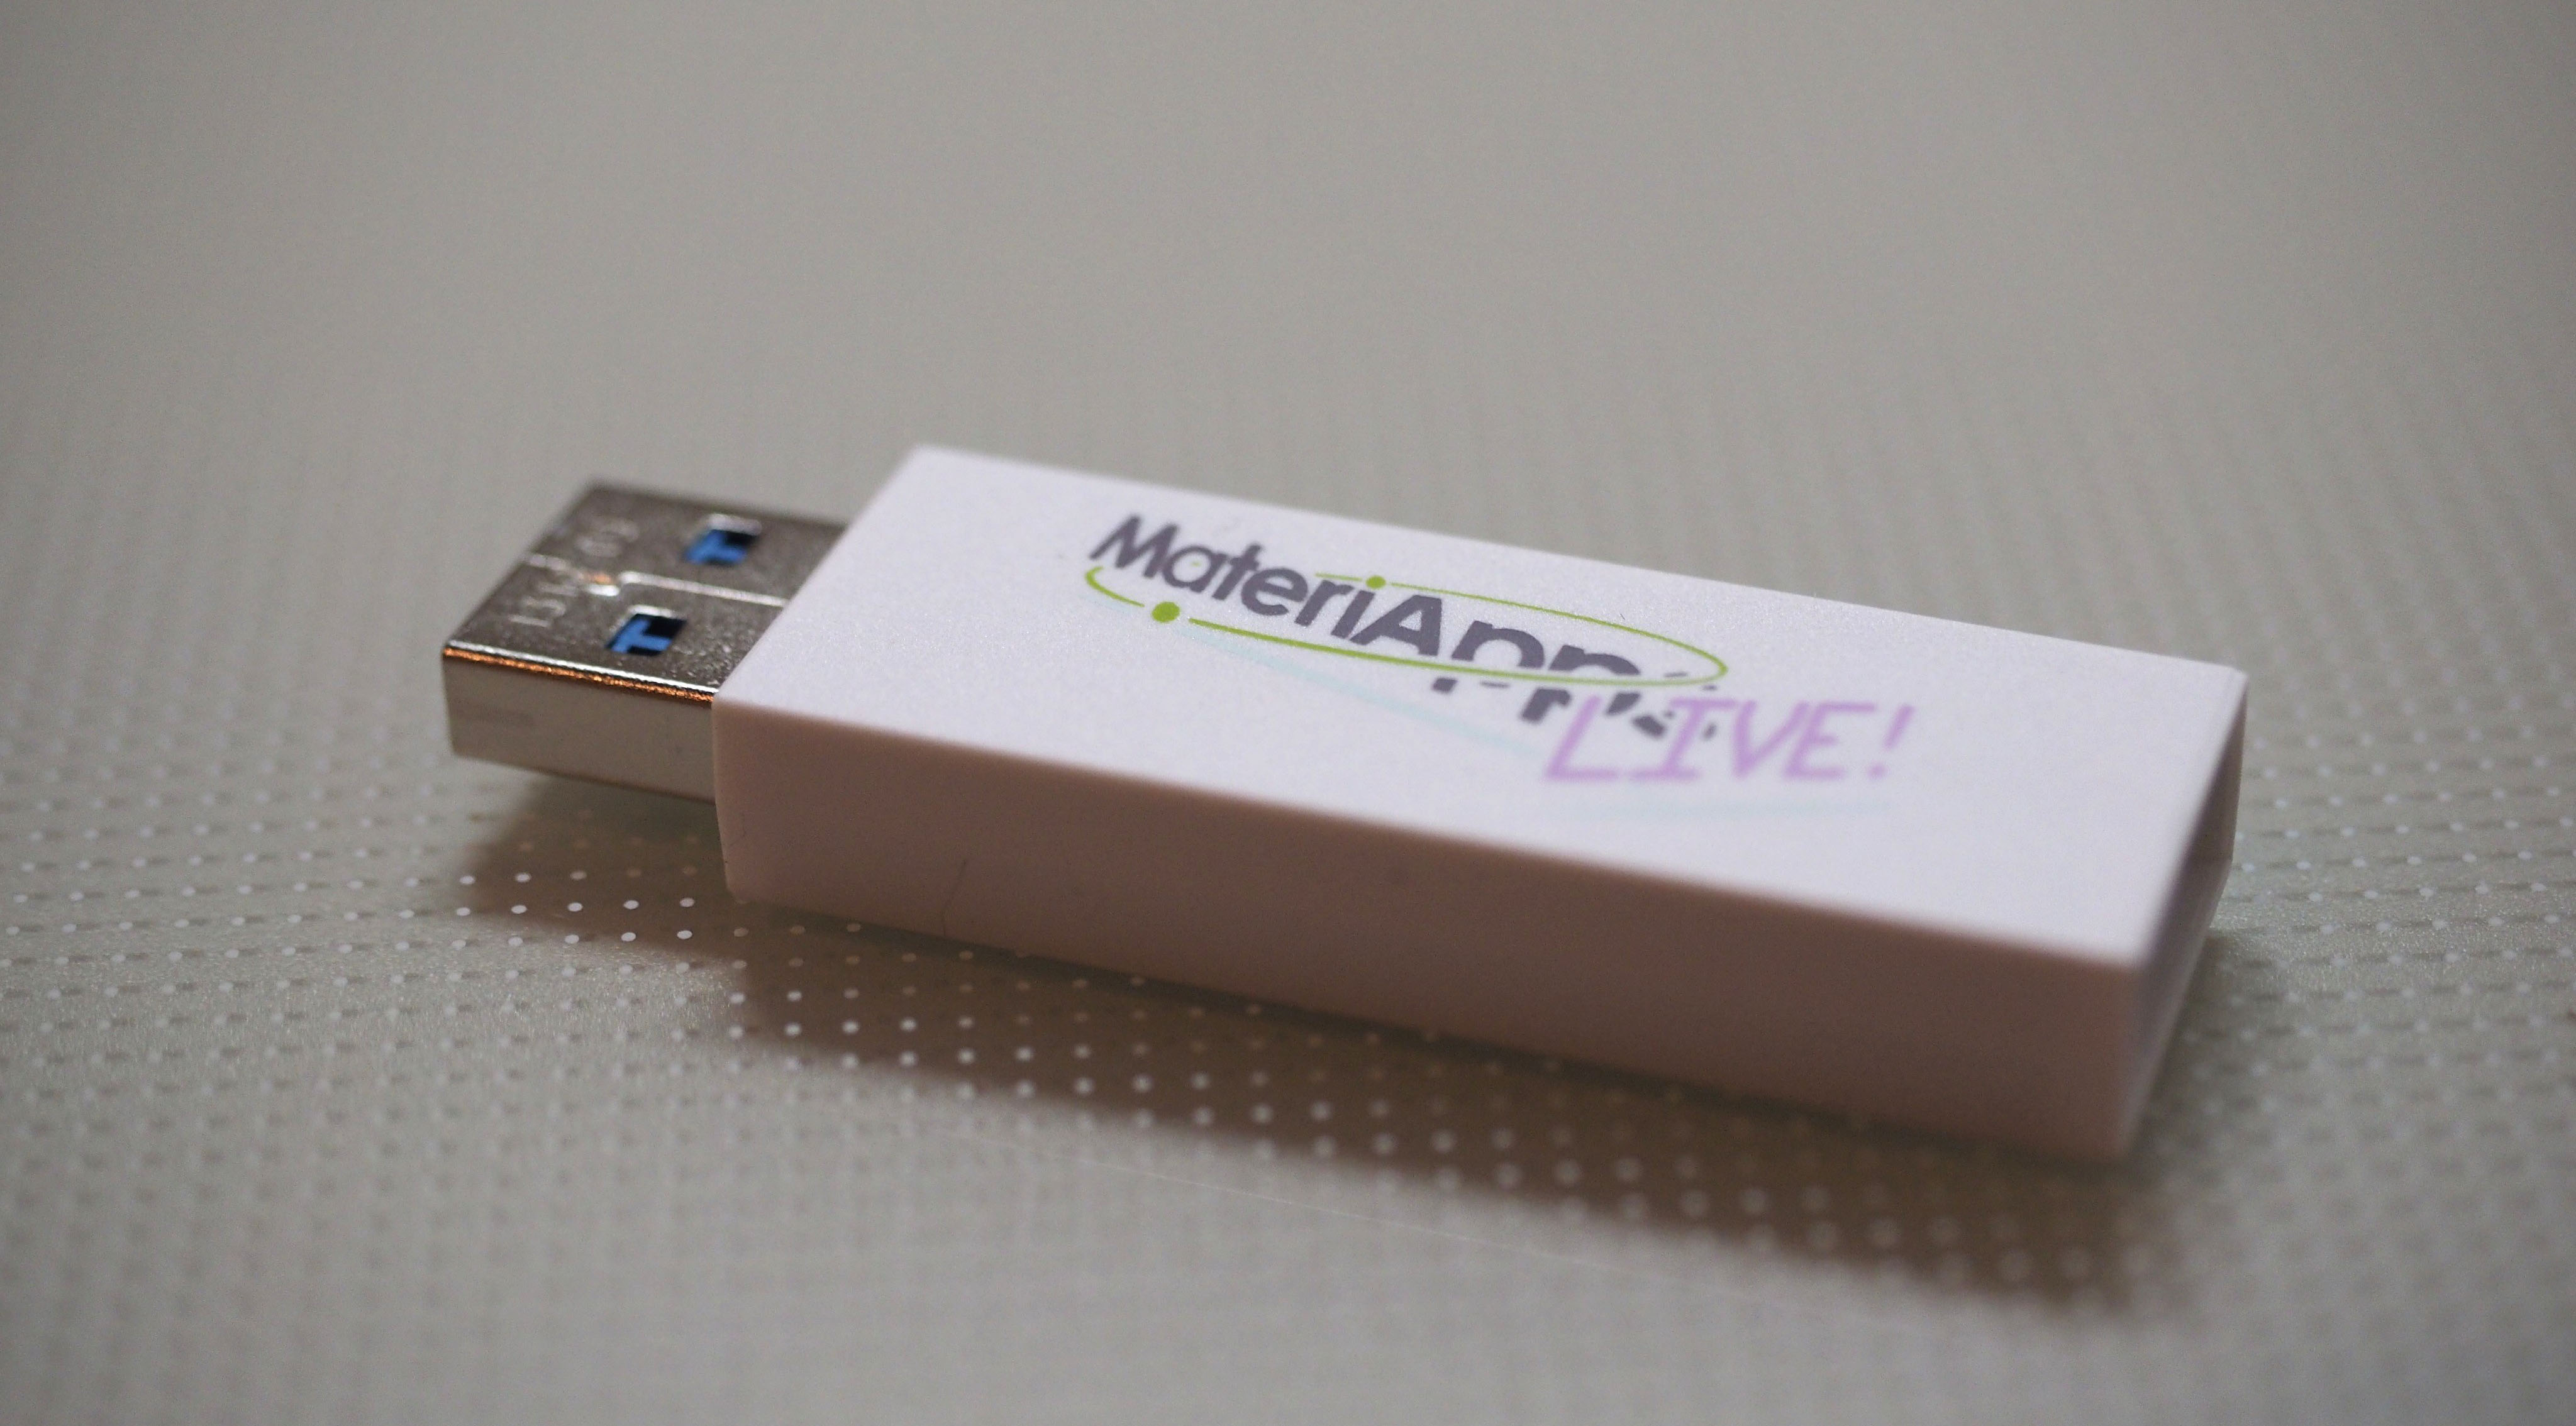
\includegraphics[width=0.3\linewidth,bb=0 0 4096 2268]{materiappslive.jpg}
     \vspace*{-1.0cm}
   \item Windows、Mac などで利用可
   \item バージョン1.2公開中
     \begin{itemize}
     \item MateriApps LIVE! サイトで配布 \url{http://cmsi.github.io/MateriAppsLive/}
     \item 学会等でも配布
     \end{itemize}
 \end{itemize}
\end{frame}

\end{document}
